 \iffalse
\let\negmedspace\undefined
\let\negthickspace\undefined
\documentclass[journal,12pt,twocolumn]{IEEEtran}
\usepackage{cite}
\usepackage{amsmath,amssymb,amsfonts,amsthm}
\usepackage{algorithmic}
\usepackage{graphicx}
\usepackage{textcomp}
\usepackage{xcolor}
\usepackage{txfonts}
\usepackage{listings}
\usepackage{enumitem}
\usepackage{mathtools}
\usepackage{gensymb}
\usepackage{comment}
\usepackage[breaklinks=true]{hyperref}
\usepackage{tkz-euclide} 
\usepackage{tikz}
% \usetikzlibrary{positioning, arrows.meta}
\usepackage{listings}
\usepackage{gvv} 
\usepackage{caption}
\def\inputGnumericTable{}                   

%\usepackage[latin1]{inputenc}                                
\usepackage{color}                                            
\usepackage{array}                                            
\usepackage{longtable}                                       
\usepackage{calc}                                             
\usepackage{multirow}                                         
\usepackage{hhline}                                           
\usepackage{ifthen}                                           
\usepackage{lscape}
\usepackage{tikz}
\newtheorem{theorem}{Theorem}[section]
\newtheorem{problem}{Problem}
\newtheorem{proposition}{Proposition}[section]
\newtheorem{lemma}{Lemma}[section]
\newtheorem{corollary}[theorem]{Corollary}
\newtheorem{example}{Example}[section]
\newtheorem{definition}[problem]{Definition}
\newcommand{\BEQA}{\begin{eqnarray}}
\newcommand{\EEQA}{\end{eqnarray}}
\newcommand{\define}{\stackrel{\triangle}{=}}
\theoremstyle{remark}
\newtheorem{rem}{Remark}

\begin{document}

\bibliographystyle{IEEEtran}
\vspace{3cm}

\title{GATE: EE - 31.2021}
\author{EE23BTECH11013 - Avyaaz$^{*}$% <-this % stops a space 
}
\maketitle
\newpage
\bigskip

\renewcommand{\thefigure}{\arabic{figure}}
\renewcommand{\thetable}{\arabic{table}}

\large\textbf{\textsl{Question:}}
The causal signal with Z transform $z^2(z - a)^{-2}$ is ($u(n)$ is unit step signal)
\begin{enumerate}
    \item $a^{2n}u(n)$
    \item $(n + 1)a^nu(n)$
    \item $n^{-1}a^nu(n)$
    \item $n^2a^nu(n)$
\end{enumerate}

\hfill(GATE EE 2021) \\
\solution
\fi
% \begin{table}[htbp]
%     \centering
%      \begin{tabular}{|c|c|c|}
\hline
    Parameter & Description & Value\\
    \hline
    $P(s)$ & Plant Transfer Function & $\frac{0.001}{s\brak{\frac{s}{0.5}+1}\brak{\frac{s}{100}+1}}$\\
    \hline
    $C(s)$ & Lag Compensator  & $\frac{100\brak{\frac{s}{10}+1}}{\frac{s}{0.1}+1}$\\
    \hline
    $T(s)$ & Loop gain  & $P(s) C(s)$ \\
    \hline
    $\omega$ & Angular Frequency & 3rad/s \\
    \hline
\end{tabular}

%     \caption{}
%     \label{tab:my_label.41.IN.2022}
% \end{table}

% \begin{figure}[!htbp]
%     \resizebox{0.501\textwidth}{!}{\documentclass{standalone}
\usepackage{tikz}
\usepackage{graphicx} % For rotatebox
\usetikzlibrary{circuits.ee.IEC}

\begin{document}
\begin{tikzpicture}[circuit ee IEC, scale=0.8, transform shape]

% Define components
\def\kone{2} % Capacitance 1/k1
\def\ktwo{3} % Capacitance 1/k2
\def\lone{1.5} % Inductance L1

% Draw parallel combination
\draw[fill=gray!30] (0,0) to [capacitor={info={$\frac{1}{k_1}$}}] ++(1.5,0) coordinate (C1)
            to [inductor={info'={$L_1$}, swap}] ++(1.5,0) coordinate (L1);

% Add parallel combination with L2 and 1/k2
\draw[fill=gray!30] (C1) ++(1.5,0) to [capacitor={info={\rotatebox{90}{$\frac{1}{k_2}$}}}] ++(0,-1.5) coordinate (C2);
\draw[fill=gray!30] (C2) ++(2,1.5) to [inductor={info'={\rotatebox{90}{$L_2$}}, swap}] ++(0,-1.5) coordinate (L2);

% Join L1 and L2 with a solid line
\draw (0,-1.5) -- (L2);
\draw (0,0) -- (0,-1.5);
\draw (3,0) --(5,0);

% Add pointer and label for i1
\draw[postaction={decorate,decoration={markings,mark=at position 0.5 with {\arrow{>}}}}] (0,0) -- node[above] {\(i_1\)} (0.5,0);

% Add pointer and label for i2
\draw[postaction={decorate,decoration={markings,mark=at position 0.5 with {\arrow{>}}}}] (3,0) -- node[above] {\(i_2\)} (3.5,0);

\end{tikzpicture}
\end{document}

}
%     \caption{Block Diagram of System}
%     \label{fig:gate_IN_Q41_blockdiagram}
% \end{figure}


Z-transform of a causal signal is, 
\begin{align}
    X(z) = z^2(z - a)^{-2} = \frac{1}{(1 - az^{-1})^2};|z| > |a|\label{eq:given.EE.31.2021}
\end{align}
The Z transform pair for $a^nu(n)$ signal is given by :
\begin{align}
    a^nu(n) \longleftrightarrow \frac{1}{1 - az^{-1}}
\end{align}
Using differentiation in z-domain property:
\begin{align}
    na^nu(n) &\longleftrightarrow -z\frac{d}{dz}\left(\frac{1}{1 - az^{-1}}\right) \\
     \implies    na^nu(n) &\longleftrightarrow \frac{az^{-1}}{(1 - az^{-1})^2}
\end{align}
Using time-shifting property:
\begin{align}
  (n + 1)a^{n + 1}u(n + 1) \longleftrightarrow \frac{az^{-1}}{(1 - az^{-1})^2}z\\
  (n + 1)a^nu(n + 1) \longleftrightarrow \frac{1}{(1 - az^{-1})^2}\label{EQ:TIME.31.EE.2021}
\end{align}
From \eqref{eq:given.EE.31.2021} and \eqref{EQ:TIME.31.EE.2021}, Inverse Z transform is :
\begin{align}
    x(n) = (n + 1)a^nu(n + 1)
\end{align}
Sequence \(u(n + 1)\) exist for\(-1 \leq n < \infty\), but the factor \((n + 1)\) is zero for \(n = -1\), so \(x(n)\) may be expressed as a causal sequence. 
\begin{align}
    x(n) = (n + 1)a^nu(n)
\end{align}



\begin{figure}[htbp]
    \centering
    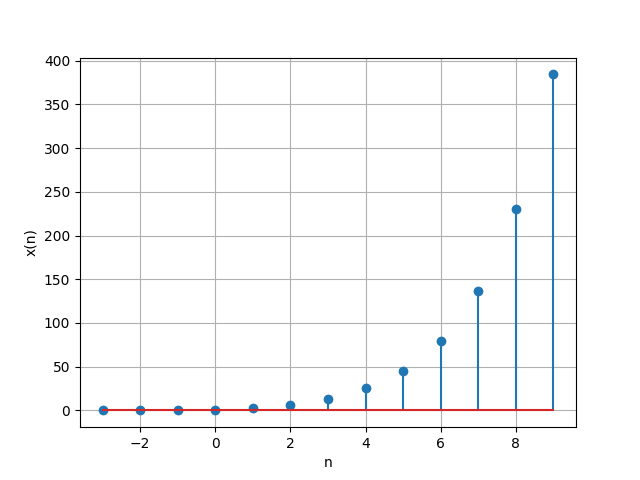
\includegraphics[width = \columnwidth]{2021/EE/31/figs/transform.png}
	\caption{$x(n) vs n $ using $a = 1.5$}
    \label{fig:graph1.41.IN.2022}
\end{figure}

